%
% teil3.tex -- Beispiel-File für Teil 3
%
% (c) 2020 Prof Dr Andreas Müller, Hochschule Rapperswil
%
\section{Beispiel einer Verfolgungskurve
\label{lambertw:section:teil4}}
\rhead{Beispiel einer Verfolgungskurve}
In diesem Abschnitt wird rechnerisch das Beispiel einer Verfolgungskurve mit der Verfolgungsstrategie 1 beschreiben. Dafür werden zuerst Bewegungsraum, Anfangspositionen und Bewegungsverhalten definiert, in einem nächsten Schritt soll eine Differentialgleichung dafür aufgestellt und anschliessend gelöst werden.

\subsection{Anfangsbedingungen definieren und einsetzen
	\label{lambertw:subsection:Anfangsbedingungen}}
Das zu verfolgende Ziel \(Z\) bewegt sich entlang der \(y\)-Achse mit konstanter Geschwindigkeit \(v = 1\), beginnend beim Ursprung des Kartesischen Koordinatensystems. Der Verfolger \(V\) startet auf einem beliebigen Punkt im ersten Quadranten und bewegt sich auch mit konstanter Geschwindigkeit \(|\dot{V}| = 1\) in Richtung Ziel. Diese Anfangspunkte oder Anfangsbedingungen können wie folgt formuliert werden:
\begin{equation}
	Z
	=
	\left( \begin{array}{c} 0 \\ v \cdot t \end{array} \right)
	=
	\left( \begin{array}{c} 0 \\ t \end{array} \right)
	,\:
	V
	=
	\left( \begin{array}{c} x \\ y \end{array} \right)
	\:\text{und}\:\:
	\bigl| \dot{V} \bigl|
	=
	1.
	\label{lambertw:Anfangsbed}
\end{equation}
Wir haben nun die Anfangsbedingungen definiert, jetzt fehlt nur noch eine DGL, welche die fortlaufende Änderung der Position und Bewegungsrichtung des Verfolgers beschreibt. 
Diese DGL haben wir bereits in Kapitel \ref{lambertw:subsection:Verfolger} definiert, und zwar Gleichung \eqref{lambertw:pursuerDGL}. Wenn man die Startpunkte einfügt, ergibt sich folgender Ausdruck:
\begin{equation}
	\frac{\left( \begin{array}{c} 0-x \\ t-y \end{array} \right)}{\sqrt{x^2 + (t-y)^2}}
	\cdot
	\left(\begin{array}{c} \dot{x} \\ \dot{y} \end{array}\right)
	=
	1.
	\label{lambertw:eqMitAnfangsbed}
\end{equation}

\subsection{Differentialgleichung vereinfachen
	\label{lambertw:subsection:DGLvereinfach}}
Nun haben wir eine Gleichung, es stellt sich aber die Frage, ob es überhaupt eine geschlossene Lösung dafür gibt. Eine Funktion welche die Beziehung \(y(x)\) beschreibt oder sogar \(x(t)\) und \(y(t)\) liefert. Zum jetzigen Zeitpunkt mag es nicht trivial scheinen, aber mit den gewählten Anfangsbedingungen \eqref{lambertw:Anfangsbed} ist es möglich eine geschlossene Lösung für die Gleichung \eqref{lambertw:eqMitAnfangsbed} zu finden.

Auf dem Weg dahin muss die definierte DGL zuerst wesentlich vereinfacht werden, sei es mittels algebraischer Umformungen oder mit den Tools aus der Analysis. Da die nächsten Schritte sehr algebralastig sind und sie das Lesen dieses Papers einfach nur mühsam machen würden, werden wir uns hier nur die wesentlichsten Schritte konzentrieren, welche notwendig sind, um den Lösungsweg nachvollziehen zu können.

\subsubsection{Skalarprodukt auflösen
	\label{lambertw:subsubsection:SkalProdAufl}}
Zuerst müssen wir den Bruch und das Skalarprodukt in \eqref{lambertw:eqMitAnfangsbed} wegbringen, damit wir eine. Dies führt zu:
\begin{equation}
		-x \cdot \dot{x} + (t-y) \cdot \dot{y}
		= \sqrt{x^2 + (t-y)^2}.
		\label{lambertw:eqOhneSkalarprod}
\end{equation}
Im letzten Schritt, fällt die Nützlichkeit des Skalarproduktes in der Verfolgungsgleichung \eqref{lambertw:pursuerDGL} markant auf. Anstatt zwei gekoppelte Differentialgleichungen zu erhalten, eine für die \(x\) und die andere für die \(y\)-Komponente, erhält man einen einzigen Ausdruck, was in der Regel mit weniger Lösungsaufwand verbunden ist.

\subsubsection{Quadrieren und Gruppieren
	\label{lambertw:subsubsection:QuadUndGrup}}
Mit der Quadratwurzel in \ref{lambertw:eqOhneSkalarprod} kann man nichts anfangen, sie steht nur im Weg, also muss man sie loswerden. Wenn man dies macht, kann \eqref{lambertw:eqOhneSkalarprod} auf folgende Form gebracht werden: 
\begin{equation}
	\left(\dot{x}^2-1\right) \cdot x^2 -2x \left(t-y\right) \dot{x}\dot{y} + \left(\dot{y}^2-1\right) \cdot \left(t-y\right)^2
	=0.
	\label{lambertw:eqOhneWurzel}
\end{equation}
Diese Form mag auf den ersten Blick nicht gerade nützlich sein, aber man kann sie mit einer Substitution weiter vereinfachen.

\subsubsection{Wichtige Substitution
	\label{lambertw:subsubsection:WichtSubst}}
Wenn man beachtet, dass die Geschwindigkeit des Verfolgers konstant und gleich 1 ist, dann kann man folgende Gleichung aufstellen: 
\begin{equation}
	\dot{x}^2 + \dot{y}^2 
	= 1.
	\label{lambertw:eqGeschwSubst}
\end{equation}
Umformungen der Gleichung \eqref{lambertw:eqGeschwSubst} können in \eqref{lambertw:eqOhneWurzel} erkannt werden. Ersetzt führen sie zu folgendem Ausdruck:
\begin{equation}
		\dot{y}^2 \cdot x^2 +2x \left(t-y\right) \dot{x}\dot{y} + \dot{x}^2 \cdot \left(t-y\right)^2
		=0.
		\label{lambertw:eqGeschwSubstituiert}
\end{equation}
Diese unscheinbare Substitution führt dazu, dass weitere Vereinfachungen durchgeführt werden können.

\subsubsection{Binom erkennen und vereinfachen
	\label{lambertw:subsubsection:BinomVereinfach}}
Versteckt im Ausdruck \eqref{lambertw:eqGeschwSubstituiert} befindet sich die erste binomische Formel, welche zu folgender Gleichung führt:
\begin{equation}
	(x \dot{y} + (t-y) \dot{x})^2
	= 0.
	\label{lambertw:eqAlgVerinfacht}
\end{equation}
Da der linke Term gleich Null ist, muss auch der Inhalt des Quadrates gleich Null sein, somit folgt eine weitere Vereinfachung, welche zu einer im Vergleich zu \eqref{lambertw:eqOhneSkalarprod} wesentlich einfacheren DGL führt:
\begin{equation}
	x \dot{y} + (t-y) \dot{x}
	= 0.
	\label{lambertw:eqGanzVerinfacht}
\end{equation}
Kompakt, ohne Wurzelterme und Quadrate, nur elementare Operationen und Ableitungen. Nun stellt sich die Frage wie es weiter gehen soll, bei der Gleichung \eqref{lambertw:eqGanzVerinfacht} scheinen keine weiteren Vereinfachungen möglich zu sein. Wir brauchen einen neuen Ansatz, um unser Ziel einer möglichen Lösung zu verfolgen.

\subsection{Zeitabhängigkeit loswerden
	\label{lambertw:subsection:ZeitabhLoswerden}}
Der nächste logischer Schritt scheint irgendwie die Zeitabhängigkeit in der Gleichung \eqref{lambertw:eqGanzVerinfacht} loszuwerden, aber wieso? Nun, wie am Anfang von Abschnitt \ref{lambertw:subsection:DGLvereinfach} beschrieben, suchen wir eine Lösung der Art \(y(x)\), dies ist natürlich erst möglich wenn wir die Abhängigkeit nach \(t\) eliminieren können.

\subsubsection{Zeitliche Ableitungen loswerden
	\label{lambertw:subsubsection:ZeitAbleit}}
Der erste Schritt auf dem Weg zur Funktion \(y(x)\), ist es die zeitlichen Ableitungen los zu werden, dafür wird \eqref{lambertw:eqGanzVerinfacht} beidseitig mit \(\dot{x}\) dividiert, was erlaubt ist, weil diese Änderung ungleich Null ist:
\begin{equation}
	x \frac{\dot{y}}{\dot{x}} + (t-y) \frac{\dot{x}}{\dot{x}}
	= 0.
	\label{lambertw:eqVorKeineZeitAbleit}
\end{equation}
Der Grund dafür ist, dass
\begin{equation}
	\frac{\displaystyle\dot{y}}{\displaystyle\dot{x}} 
	= \frac{\displaystyle\frac{dy}{dt}}{\displaystyle\frac{dx}{dt}}  
	= \frac{dy}{dx}
	= y^{\prime},
	\label{lambertw:eqQuotZeitAbleit}
\end{equation}
und somit kann der Quotient dieser zeitlichen Ableitungen in eine Ableitung nach \(x\) umgewandelt werden.
Nach dem die Eigenschaft \eqref{lambertw:eqQuotZeitAbleit} in \eqref{lambertw:eqVorKeineZeitAbleit} eingesetzt wird und vereinfacht wurde, entsteht die neue Gleichung
\begin{equation}
	x y^{\prime} + t - y
	= 0.
	\label{lambertw:DGLmitT}
\end{equation}

\subsubsection{Variable \(t\) eliminieren
	\label{lambertw:subsubsection:ZeitAbleit}}
Hier wäre es natürlich passend, wenn man die Abhängigkeit nach \(t\) komplett wegbringen könnte. Um dies zu erreichen, muss man auf die Definition der Bogenlänge zurückgreifen. 
Die Strecke \(s\) entspricht 
\begin{equation}
	s
	= 
	v \cdot t
	=
	1 \cdot t
	=
	t
	=
	\int_{\displaystyle x_0}^{\displaystyle x_{\text{end}}}\sqrt{1+y^{\prime\, 2}} \: dx.
	\label{lambertw:eqZuBogenlaenge}
\end{equation}

Nicht gerade auffällig ist die Richtung, in welche hier integriert wird. Wenn der Verfolger sich wie vorgesehen am Anfang im ersten Quadranten befindet, dann muss sich dieser nach links bewegen, was nicht der üblichen Integrationsrichtung entspricht. Um eine Integration wie üblich von links nach rechts ausführen zu können, müssen die Integrationsgenerzen vertauscht werden, was in einem Vorzeichenwechsel resultiert. 

Wenn man nun \eqref{lambertw:eqZuBogenlaenge} in die DGL \eqref{lambertw:DGLmitT} einfügt, dann ergibt sich folgender Ausdruck:
\begin{equation}
	x y^{\prime} - \int\sqrt{1+y^{\prime\, 2}} \: dx - y
	= 0.
	\label{lambertw:DGLohneT}
\end{equation}
Um das Integral los zu werden, leitet man den vorherigen Ausdruck \eqref{lambertw:DGLohneT} nach \(x\) ab und erhaltet folgende DGL zweiter Ordnung \eqref{lambertw:DGLohneInt}:
\begin{align}
	y^{\prime}+ xy^{\prime\prime} - \sqrt{1+y^{\prime\, 2}} - y^{\prime}
	&= 0, \\
	xy^{\prime\prime} - \sqrt{1+y^{\prime\, 2}}
	&= 0.
	\label{lambertw:DGLohneInt}
\end{align}
Nun sind wir unserem Ziel einen weiteren Schritt näher. Die Gleichung \eqref{lambertw:DGLohneInt} mag auf den ersten Blick nicht gerade einfach sein, aber im Nächsten Abschnitt werden wir sehen, dass sie relativ einfach zu lösen ist.

\subsection{Differentialgleichung lösen
	\label{lambertw:subsection:DGLloes}}
Die Gleichung \eqref{lambertw:DGLohneInt} ist eine DGL zweiter Ordnung, in der \(y\) nicht vorkommt. Sie kann mittels der Substitution \(y^{\prime} = u\) in eine DGL erster Ordnung umgewandelt werden:
\begin{equation}
	xu^{\prime} - \sqrt{1+u^2}
	= 0.
	\label{lambertw:DGLmitU}
\end{equation}
Diese Gleichung ist separierbar, was sie viel handlicher macht. In der separierten Form
\begin{equation}
	\int{\frac{1}{\sqrt{1+u^2}}\:du} 
	= 
	\int{\frac{1}{x}\:dx},
\end{equation}
lässt sich die Gleichung mittels einer Integrationstabelle sehr rasch lösen. 
Mit dem Ergebnis: 
\begin{align}
	\operatorname{arsinh}(u)
	&=
	\operatorname{ln}(x) + C, \\
	u
	&=
	\operatorname{sinh}(\operatorname{ln}(x) + C).
	\label{lambertw:loesDGLmitU}
\end{align}
Wenn man in \eqref{lambertw:loesDGLmitU} die Substitution rückgängig macht, erhält man folgende DGL erster Ordnung, die bereits separiert ist:
\begin{equation}
	y^{\prime}
	=
	\operatorname{sinh}(\operatorname{ln}(x) + C).
	\label{lambertw:loesDGLmitY}
\end{equation}
Ersetzt man den \(\operatorname{sinh}\) mit seiner exponentiellen Definition \(\operatorname{sinh}(x)=\frac{1}{2}(e^x-e^{-x})\), so resultiert auf sehr einfache Art folgende Lösung für \eqref{lambertw:loesDGLmitY}:
\begin{equation}
	y
	=
	C_1 + C_2 x^2 - \frac{\operatorname{ln}(x)}{8 \cdot C_2}.
\end{equation}
Nun haben wir eine Lösung, aber wie es immer mit Lösungen ist, stellt sich die Frage, ob sie überhaupt plausibel ist. Dieser Frage werden wir im nächsten Abschnitt nachgehen.

\subsection{Lösung analysieren
	\label{lambertw:subsection:LoesAnalys}}

\begin{figure}
	\centering
	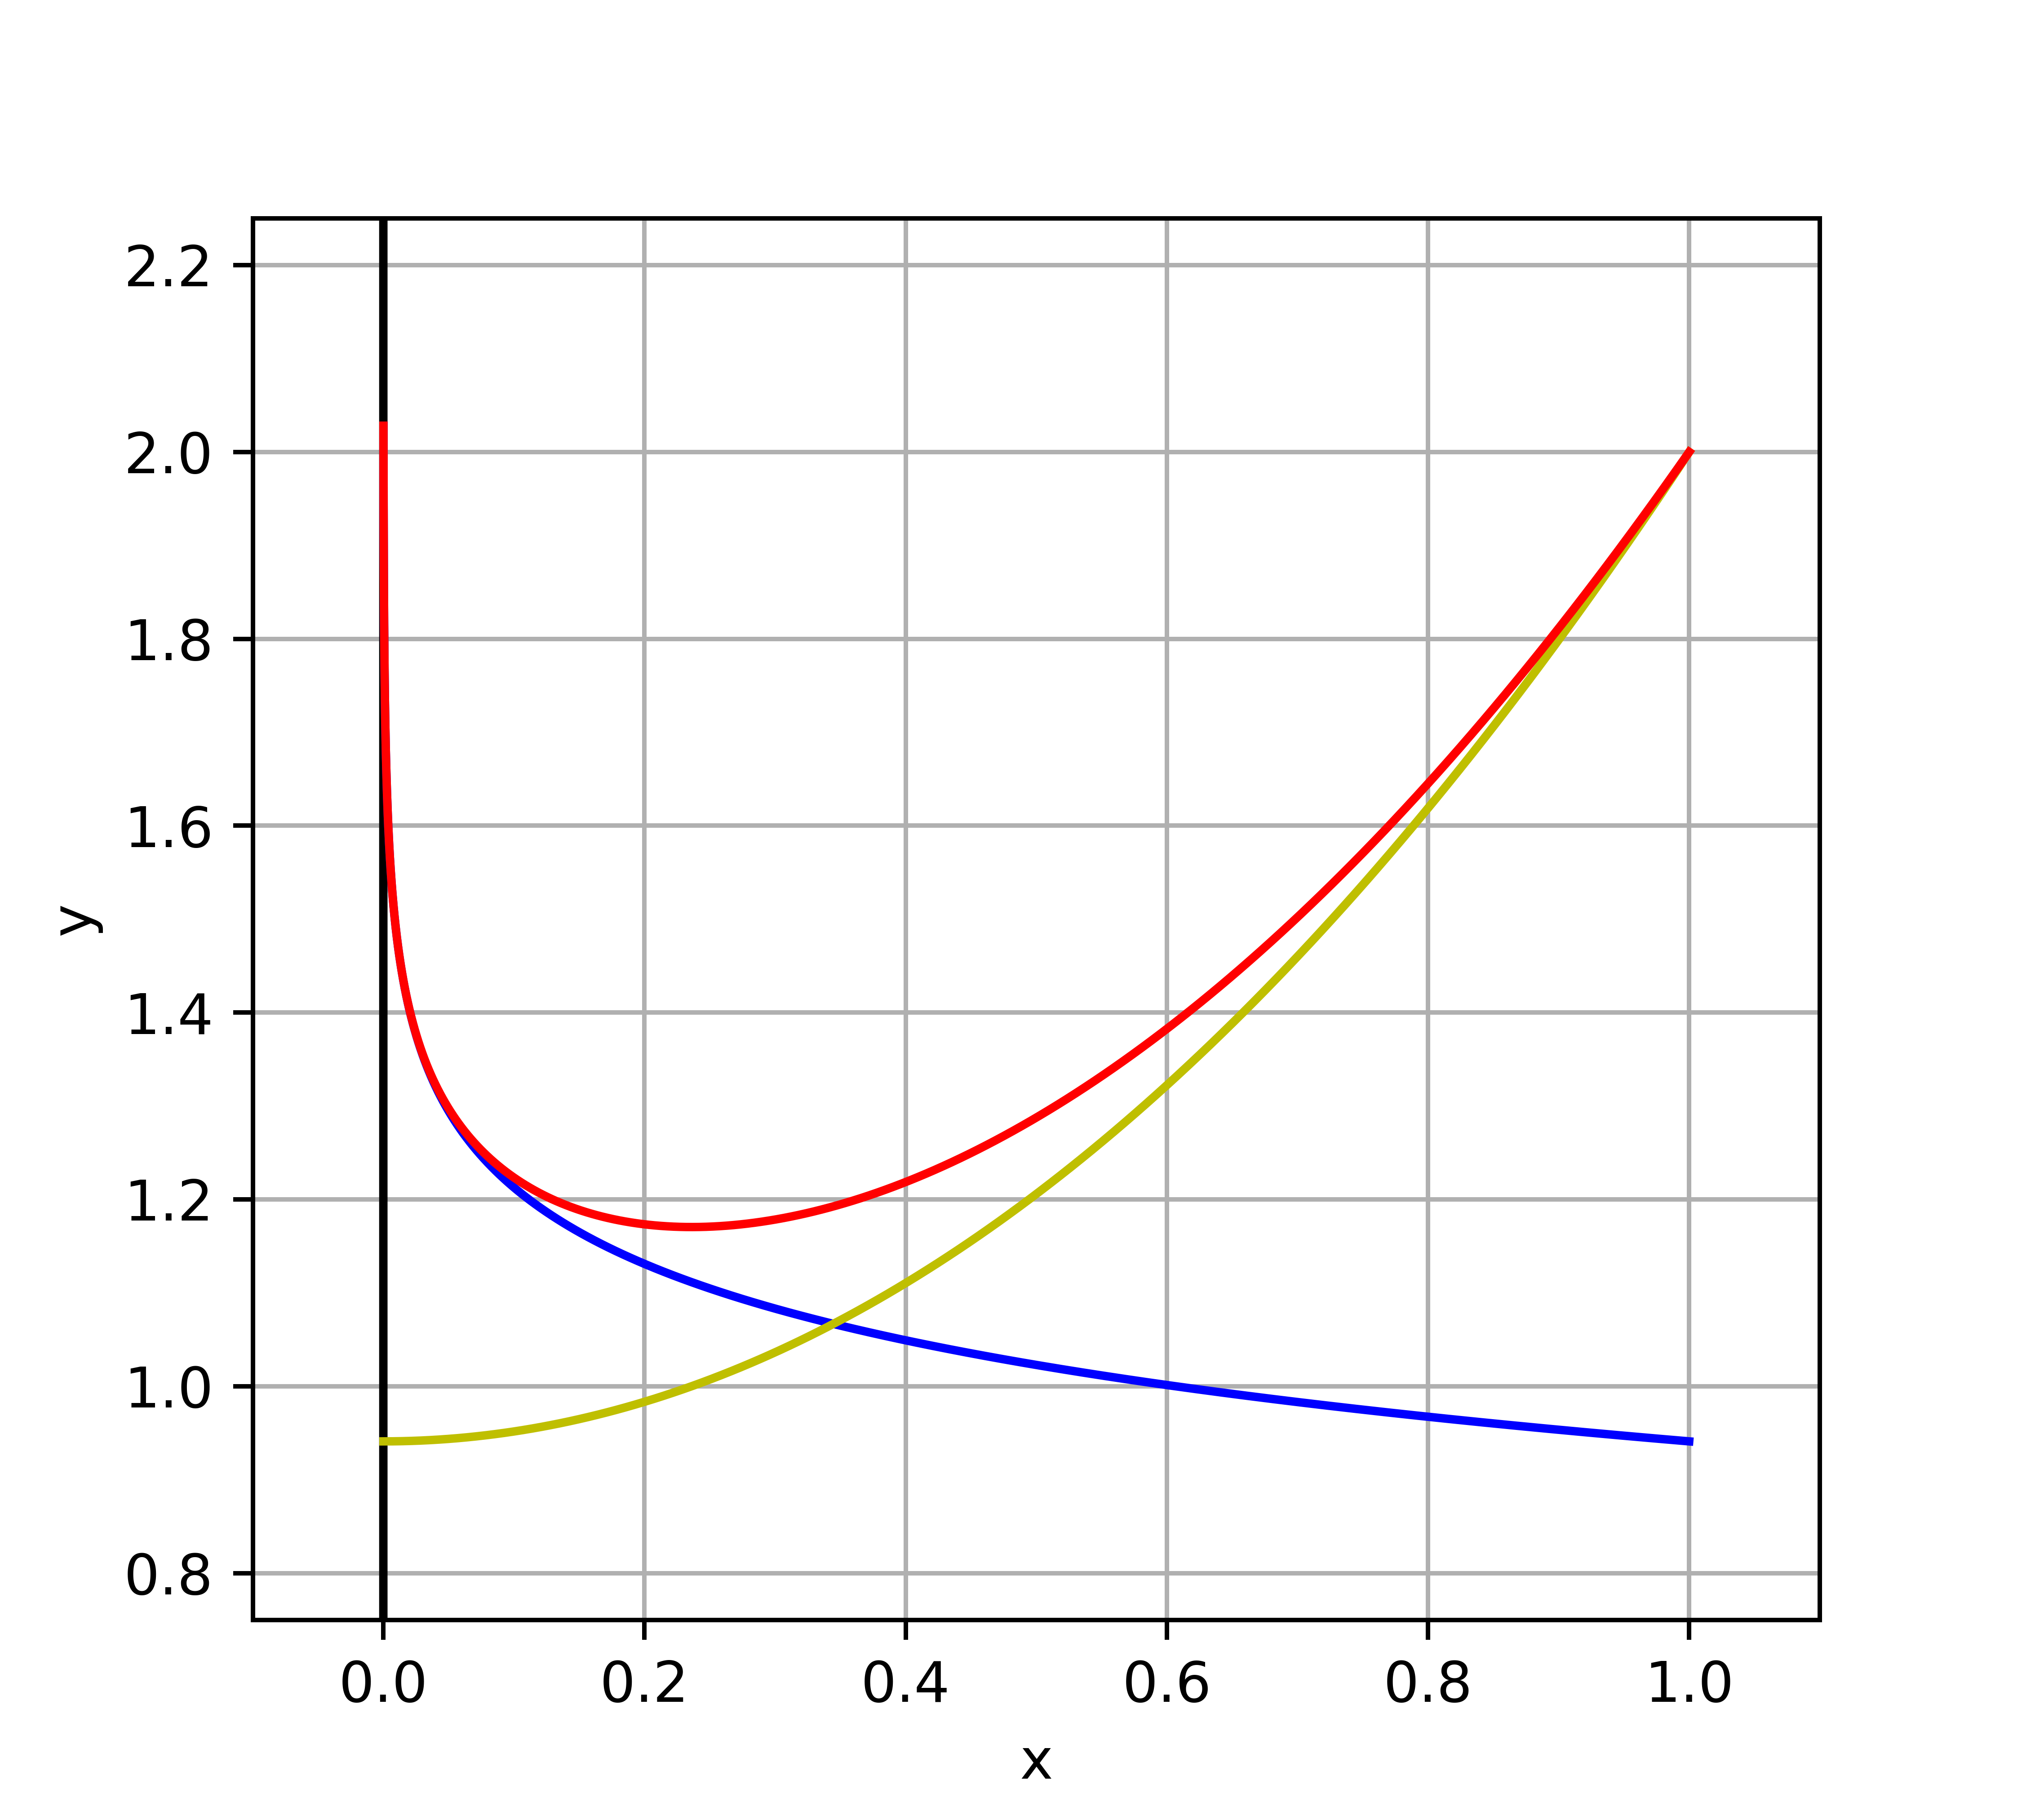
\includegraphics{papers/lambertw/Bilder/VerfolgungskurveBsp.png}
	\caption[Graph der Verfolgungskurve]{Graph der Verfolgungskurve wobei, ({\color{red}rot}) die Funktion \ensuremath{y(x)} ist, ({\color{darkgreen}grün}) der quadratische Teil und ({\color{blue}blau}) dem \ensuremath{\operatorname{ln}(x)}-Teil entspricht.
	\label{lambertw:BildFunkLoes}
	}
\end{figure}

Das Resultat, wie ersichtlich, ist folgende Funktion \eqref{lambertw:funkLoes} welche mittels Anfangsbedingungen parametrisiert werden kann: 
\begin{equation}
	{\color{red}{y(x)}}
	=
	C_1 + C_2 {\color{darkgreen}{x^2}} {\color{blue}{-}} \frac{\color{blue}{\operatorname{ln}(x)}}{8 \cdot C_2}.
	\label{lambertw:funkLoes}
\end{equation}
Für die Koeffizienten \(C_1\) und \(C_2\) ergibt sich ein Anfangswertproblem, welches für deren Bestimmung gelöst werden muss. Zuerst soll aber eine qualitative Intuition oder Idee für das Aussehen der Funktion \(y(x)\) geschaffen werden:
\begin{itemize}
	\item
	Für grosse \(x\)-Werte, welche in der Regel in der Nähe von \(x_0\) sein sollten, ist der quadratisch Term in der Funktion \eqref{lambertw:funkLoes} dominant. 
	\item
	Für immer kleiner werdende \(x\) geht der Verfolger in Richtung \(y\)-Achse, wobei seine Steigung stetig sinkt, was Sinn macht wenn der Verfolgte entlang der \(y\)-Achse steigt. Irgendwann werden Verfolger und Ziel auf gleicher Höhe sein, also gleiche \(y\) aber verschiedene \(x\)-Koordinate besitzen.
	\item
	Für \(x\)-Werte in der Nähe von \(0\) ist das asymptotische Verhalten des Logarithmus dominant, dies macht auch Sinn, da sich der Verfolgte auf der \(y\)-Achse bewegt und der Verfolger ihm nachgeht.
	\item
	Aufgrund des Monotoniewechsels in der Kurve \eqref{lambertw:funkLoes} muss diese auch ein Minimum aufweisen. Es stellt sich nun die Frage: Wo befindet sich dieser Punkt? 
	Eine Abschätzung darüber kann getroffen werden und zwar, dass dieser dann entsteht, wenn \(A\) und \(P\) die gleiche \(y\)-Koordinaten besitzen. In diesem Moment ändert die Richtung der \(y\)-Komponente der Geschwindigkeit des Verfolgers, somit auch sein Vorzeichen und dadurch entsteht auch das Minimum.
\end{itemize}
Alle diese Eigenschaften stimmen mit dem überein, was man von einer Kurve dieser Art erwarten würde, welche durch die Grafik \ref{lambertw:BildFunkLoes} repräsentiert wurde.

\subsection{Anfangswertproblem 
	\label{lambertw:subsection:AllgLoes}}
In diesem Abschnitt soll eine Parameterfunktion hergeleitet werden, bei der jeder beliebige Anfangspunkt im ersten Quadranten eingesetzt werden kann, ausser der Ursprung im Koordinatensystem. Diese Aufgabe erfordert ein Anfangswertproblem.

Das Lösen des Anfangswertproblems ist ein Problem aus der Algebra, auf welches hier nicht explizit eingegangen wird. Zur Vollständigkeit und Nachvollziehbarkeit, wird aber das Gleichungssystem präsentiert, welches notwendig ist, um das Anfangswertproblem zu lösen.

\subsubsection{Anfangswerte bestimmen
	\label{lambertw:subsubsection:Anfangswerte}}
Der erste Schritt auf dem Weg zur gesuchten Parameterfunktion ist, die Anfangswerte \eqref{lambertw:eq1Anfangswert} zu definieren.
Die Anfangswerte sind:
\begin{equation}
	y(x)\big \vert_{t=0}
	=
	y(x_0)
	= 
	y_0
	\label{lambertw:eq1Anfangswert}
\end{equation}
und
\begin{equation}
	\frac{dy}{dx}\bigg \vert_{t=0}
	=
	y^{\prime}(x_0)
	=
	\frac{y_0}{x_0}.
	\label{lambertw:eq2Anfangswert}
\end{equation}
Der zweite Anfangswert \eqref{lambertw:eq2Anfangswert} mag nicht grade offensichtlich sein. Die Erklärung dafür ist aber simpel: Der Verfolger wird sich zum Zeitpunkt \(t=0\) in Richtung Koordinatenursprung bewegen wollen, wo sich das Ziel befindet. Somit entsteht das Steigungsdreieck mit \(\Delta x = x_0\) und \(\Delta y = y_0\).

\subsubsection{Gleichungssystem aufstellen und lösen
	\label{lambertw:subsubsection:GlSys}}
Wenn man die Anfangswerte \eqref{lambertw:eq1Anfangswert} und \eqref{lambertw:eq2Anfangswert} in die Gleichung \eqref{lambertw:funkLoes} und deren Ableitung \(y^{\prime}(x)\) einsetzt, dann ergibt sich folgendes Gleichungssystem:
\begin{subequations}
	\begin{align}
		y_0
		&=
		C_1 + C_2 x^2_0 - \frac{\operatorname{ln}(x_0)}{8 \cdot C_2}, \\
		\frac{y_0}{x_0}
		&=
		2 \cdot  C_2 x_0 - \frac{1}{8 \cdot C_2 \cdot x_0}.
	\end{align}
	\label{lambertw:eqGleichungssystem}
\end{subequations}
Damit die gesuchte Funktion im ersten Quadranten bleibt, werden nur die positiven Lösungen des Gleichungssystems gewählt, welche wie folgt aussehen:
\begin{subequations}
	\begin{align}
		\label{lambertw:eqKoeff1}
		C_1
		&=
		\frac{2\cdot\operatorname{ln}(x_0)\left(\sqrt{x_0^2 + y_0^2} - y_0 \right) - \sqrt{x_0^2 + y_0^2} + 3 y_0}{4}, \\
		\label{lambertw:eqKoeff2}
		C_2
		&=
		\frac{\sqrt{x_0^2 + y_0^2} + y_0}{4x_0^2}.
	\end{align}
\end{subequations}
\subsubsection{Gesuchte Parameterfunktion aufstellen
	\label{lambertw:subsubsection:ParamFunk}}
Wenn man die Koeffizienten \eqref{lambertw:eqKoeff1} und \eqref{lambertw:eqKoeff2} in die Funktion \eqref{lambertw:funkLoes} einsetzt, dann ergibt sich nach dem Vereinfachen die gesuchte Parameterfunktion:
\begin{equation}
	y(x)
	=
	\frac{1}{4}\left(\left(y_0+r_0\right)\eta+\left(r_0-y_0\right)\operatorname{ln}\left(\eta\right)-r_0+3y_0\right).
	\label{lambertw:eqAllgLoes}
\end{equation}
Damit die Funktion \eqref{lambertw:eqAllgLoes} trotzdem übersichtlich bleibt, wurden Anfangssteigung \(\eta\) und Anfangsentfernung \(r_0\) wie folgt definiert:
\begin{equation}
	\eta
	=
	\left(\frac{x}{x_0}\right)^2
	\:\:\text{und}\:\:
	r_0
	=
	\sqrt{x_0^2+y_0^2}.
\end{equation}
Diese neue allgemeine Funktion \eqref{lambertw:eqAllgLoes} weist immer noch die selbe Struktur wie die vorher hergeleitete Funktion \eqref{lambertw:funkLoes} auf. Sie enthält einerseits einen quadratischen Teil, der in \(\eta\) enthalten ist, anderseits den \(\operatorname{ln}\)-Teil. Aus dieser Ähnlichkeit kann geschlossen werden, dass sich \eqref{lambertw:eqAllgLoes} auf eine ähnliche Art verhalten wird.

Nun sind wir soweit, dass wir eine \(y(x)\)-Beziehung für beliebige Anfangswerte darstellen können, unser erstes Ziel wurde erreicht. Wir können aber einen Schritt weiter gehen und uns Fragen: Ist es analytisch möglich herauszufinden, wo sich Verfolger und Ziel zu jedem Zeitpunkt befinden? Dieser Frage werden wir im nächsten Abschnitt nachgehen.

\subsection{Funktion nach der Zeit 
	\label{lambertw:subsection:FunkNachT}}
In diesem Abschnitt werden algebraischen Umformungen ein wenig detaillierter als zuvor beschrieben. Dies hat auch einen bestimmten Grund: Den Einsatz einer speziellen Funktion aufzeigen, sowie auch wann und wieso diese vorkommt. Welche spezielle Funktion? Fragst du dich wahrscheinlich in diesem Moment. Nun, um diese Frage kurz zu beantworten, es ist ``YouTube's favorite special function'' laut dem Mathematiker Michael Penn, die Lambert-\(W\)-Funktion \(W(x)\) welche im Kapitel \ref{buch:section:lambertw} bereits beschrieben wurde.

\subsubsection{Zeitabhängigkeit wiederherstellen
	\label{lambertw:subsubsection:ZeitabhWiederherst}}
Der erste Schritt ist es herauszufinden, wie die Zeitabhängigkeit wieder hineingebracht werden kann. Dafür greifen wir auf die letzte Gleichung zu, in welcher \(t\) noch enthalten war, und zwar DGL \eqref{lambertw:DGLmitT}, welche zur Übersichtlichkeit hier nochmals aufgeführt wird:
\begin{equation}
	x y^{\prime} + t - y
	= 0.
	\label{lambertw:eqDGLmitTnochmals}
\end{equation}
Wie in \eqref{lambertw:eqDGLmitTnochmals} zu sehen ist, werden \(y\) und deren Ableitung \(y^{\prime}\) benötigt, diese sind:
\begin{subequations}
	\begin{align}
		y
		&=
		\frac{1}{4}\left(\left(y_0+r_0\right)\eta+\left(r_0-y_0\right)\operatorname{ln}\left(\eta\right)-r_0+3y_0\right), \\
		\label{lambertw:eqFunkUndAbleit1}
		y^\prime
		&=
		\frac{1}{2}\left(\left(y_0+r_0\right)\frac{x}{x_0^2}+\left(r_0-y_0\right)\frac{1}{x}\right).
	\end{align}
	\label{lambertw:eqFunkUndAbleit}
\end{subequations}

Wenn man diese Gleichungen \ref{lambertw:eqFunkUndAbleit} in die DGL \label{lambertw:eqDGLmitTnochmals} einfügt, vereinfacht und nach \(t\) auflöst, dann ergibt sich folgenden Ausdruck:
\begin{equation}
	-4t
	=
	\left(y_0+r_0\right)\left(\eta-1\right)+\left(r_0-y_0\right)\operatorname{ln}\left(\eta\right).
	\label{lambertw:eqFunkUndAbleitEingefuegt}
\end{equation}

\subsubsection{Umformungen die zur Funktion nach der Zeit führen
	\label{lambertw:subsubsection:UmformBisZumZiel}}
Mit dem Ausdruck \eqref{lambertw:eqFunkUndAbleitEingefuegt}, welcher Terme mit \(x\) und \(t\) verbindet, kann nun nach der gesuchten Variable \(x\) aufgelöst werden. 


In einem nächsten Schritt wird alles mit \(x\) auf die eine Seite gebracht, der Rest auf die andere Seite und anschliessend beidseitig exponentiert, was wie folgt aussieht:
\begin{align}
	-4t+\left(y_0+r_0\right)
	&=
	\left(y_0+r_0\right)\eta+\left(r_0-y_0\right)\operatorname{ln}\left(\eta\right), \\
	e^{\displaystyle -4t+\left(y_0+r_0\right)}
	&=
	e^{\displaystyle \left(y_0+r_0\right)\eta}\cdot\eta^{\displaystyle \left(r_0-y_0\right)}.
	\label{lambertw:eqMitExp}
\end{align}
Auf dem rechten Term von \eqref{lambertw:eqMitExp} beginnen wir langsam eine ähnliche Struktur wie \(\eta e^\eta\) zu erkennen, dies schreit nach der Struktur die benötigt wird um \(\eta\) mittels der Lambert-\(W\)-Funktion \(W(x)\) zu erhalten. Dies macht durchaus Sinn, wenn wir die Funktion \(x(t)\) finden wollen und \(W(x)\) die Umkehrfunktion von \(x e^x\) ist. 

Die erste Sache die uns in \eqref{lambertw:eqMitExp} stört ist, dass \(\eta\) als Potenz da steht. Dieses Problem können wir loswerden, indem wir beidseitig mit \(\:\displaystyle \frac{1}{r_0-y_0}\:\) potenzieren:
\begin{equation}
	e^{\displaystyle \frac{-4t}{r_0-y_0}+\frac{y_0+r_0}{r_0-y_0}}
	=
	\eta\cdot e^{\displaystyle \frac{y_0+r_0}{r_0-y_0}\eta} .
	\label{lambertw:eqOhnePotenz}
\end{equation}
Das nächste Problem auf welches wir in \eqref{lambertw:eqOhnePotenz} treffen ist, dass \(\eta\) nicht alleine im Exponent steht. Dies kann elegant mit folgender Substitution gelöst werden:
\begin{equation}
	\chi
	=
	\frac{y_0+r_0}{r_0-y_0}.
	\label{lambertw:eqChiSubst}
\end{equation}
Es gäbe natürlich andere Substitutionen wie z.B. 
\[\displaystyle \chi=\frac{y_0+r_0}{r_0-y_0}\cdot\eta,\] 
die auf dasselbe Ergebnis führen würden, aber \eqref{lambertw:eqChiSubst} liefert in einem Schritt die kompakteste Lösung. Also fahren wir mit der Substitution \eqref{lambertw:eqChiSubst} weiter, setzen diese in die Gleichung \eqref{lambertw:eqOhnePotenz} ein und multiplizieren beidseitig mit \(\chi\). Daraus erhalten wir folgende Gleichung:
\begin{equation}
	\chi\cdot e^{\displaystyle \chi-\frac{4t}{r_0-y_0}}
	=
	\chi\eta\cdot e^{\displaystyle \chi\eta}.
	\label{lambertw:eqNachSubst}
\end{equation}
Nun sind wir endlich soweit, dass wir die angedeutete Lambert-\(W\)-Funktion \(W(x)\)einsetzen können. Wenn wir beidseitig \(W(x)\) anwenden, dann erhalten wir folgenden Ausdruck:
\begin{equation}
	W\left(\chi\cdot e^{\displaystyle \chi-\frac{4t}{r_0-y_0}}\right)
	=
	\chi\eta.
\end{equation}
Nach dem Auflösen nach \(x\) welches in \(\eta\) enthalten ist, erhalten wir die gesuchte \(x(t)\)-Funktion \eqref{lambertw:eqFunkXNachT}. Dieses \(x(t)\) in Kombination mit \eqref{lambertw:eqFunkUndAbleit1} liefert die Position des Verfolgers zu jedem Zeitpunkt. Das Gleichungspaar \eqref{lambertw:eqFunktionenNachT}, besteht aus folgenden Gleichungen:
\begin{subequations}
	\begin{align}
		\label{lambertw:eqFunkXNachT}
		x(t)
		&=
		x_0\cdot\sqrt{\frac{W\left(\chi\cdot e^{\displaystyle \chi-\frac{4t}{r_0-y_0}}\right)}{\chi}}, \\
		\label{lambertw:eqFunkYNachT}
		y(x(t))
		=
		y(t)
		&=
		\frac{1}{4}\left(\left(y_0+r_0\right)\left(\frac{x(t)}{x_0}\right)^2+\left(r_0-y_0\right)\operatorname{ln}\left(\left(\frac{x(t)}{x_0}\right)^2\right)-r_0+3y_0\right).
	\end{align}
	\label{lambertw:eqFunktionenNachT}
\end{subequations}
Nun haben wir unser letztes Ziel erreicht und sind in der Lage eine Verfolgung rechnerisch sowie graphisch zu repräsentieren.

\subsubsection{Hinweise zur Lambert-\(W\)-Funktion
	\label{lambertw:subsubsection:HinwLambertW}}
Wir sind aber noch nicht ganz fertig, eine Frage muss noch beantwortet werden. Und zwar wieso, dass man schon bei der Gleichung \eqref{lambertw:eqFunkUndAbleitEingefuegt} weiss, dass die Lambert-\(W\)-Funktion zum Einsatz kommen wird.
Nun, der Grund dafür ist die Struktur
\begin{equation}
	y
	=
	p(x) +\operatorname{ln}(x),
	\label{lambertw:eqEinsatzLambW}
\end{equation}
bei welcher \(p(x)\) eine beliebige Potenz von \(x\) darstellt. 

Jedes Mal wenn \(x\) gesucht ist und in einer Struktur der Art \eqref{lambertw:eqEinsatzLambW} vorkommt, dann kann mit ein paar Umformungen die Struktur \(f(x)e^{f(x)}\) erzielt werden. Wie bereits in diesem Abschnitt \ref{lambertw:subsection:FunkNachT} gezeigt wurde, kann \(x\) nun mittels der \(W(x)\)-Funktion aufgelöst werden. Erstaunlicherweise ist \eqref{lambertw:eqEinsatzLambW} eine Struktur die oftmals vorkommt, was die Lambert-\(W\)-Funktion so wichtig macht.